\documentclass[11pt,class=report,crop=false]{standalone}
\usepackage[screen]{../python}

\pagestyle{empty}

\begin{document}

% Commande spécifique
\newcommand{\badletter}[1]{\underline{\textcolor{red}{#1}}}



%====================================================================
\chapitre{Statistique -- Visualisation de données}
%====================================================================

\newpage

    \section*{Somme}
    
  \begin{fonctionpython}[\ci{python : sum()}]
   Usage : \ci{sum(liste)}\\
   Entrée : une liste de nombres\\
   Sortie : un nombre
  
  \medskip
     
   Exemple : \ci{sum([4,8,3])} renvoie \ci{15}
  \end{fonctionpython}   

\newpage  
    \section*{Minimum/maximum}  
    
    
  \begin{fonctionpython}[\ci{python : min()}]
   Usage : \ci{min(liste)} \  ou \  \ci{min(a,b)}\\
   Entrée : une liste de nombres ou bien deux nombres\\
   Sortie : un nombre
  
  \medskip
     
   Exemple : 
  \begin{itemize}  
    \item \ci{min(12,7)} renvoie \ci{7}  
    \item \ci{min([10,5,9,12])} renvoie \ci{5}
  \end{itemize}    

  \end{fonctionpython}   
  
\newpage 
 
  \section*{Variance et écart-type}
  
 La \defi{variance}\index{variance} d'une série de données $(x_1,x_2,\ldots,x_n)$ est définie comme la moyenne des carrés des écarts à la moyenne. C'est-à-dire :
  $$v = \frac{1}{n}\big((x_1-m)^2 + (x_2-m)^2 + \cdots + (x_n-m)^2\big)$$
  où $m$ est la moyenne de $(x_1,x_2,\ldots,x_n)$.
  
  \bigskip  
  
  Par exemple, pour la série $(6,8,2,10)$, la moyenne est $m = 6.5$, la variance est
  $$v = \frac{1}{4} \big((6-6.5)^2 + (8-6.5)^2 + (2-6.5)^2 + (10-6.5)^2\big) = 8.75$$
  
  \bigskip
   
  \bigskip
   
   L'\defi{écart-type}\index{ecart-type@écart-type} d'une série $(x_1,x_2,\ldots,x_n)$ est la racine carrée de la variance :
  $$e = \sqrt{v}$$
  où $v$ est la variance.
  
   \bigskip 
   Exemple :
    $$e = \sqrt{v} = \sqrt{8.75} = 2.95\ldots $$

%%%%%%%%%%%%%%%%%%%%%%%%%%%%%%%%%%%%%%%%%%%%%%%%%%%%%%%%%%%%%%%%
%%%%%%%%%%%%%%%%%%%%%%%%%%%%%%%%%%%%%%%%%%%%%%%%%%%%%%%%%%%%%%%%

\newpage

\section*{Graphiques avec tkinter}


\myfigure{0.8}{
\tikzinput{fig-stat-cours-intro}
}


\begin{itemize}

  \item \ci{create_rectangle(x1,y1,x2,y2)}
  
  \item  \ci{create_oval(x1,y1,x2,y2)}
  
  \item \ci{create_text(x,y,text="Mon texte")} 
  
\end{itemize}


\newpage

\section*{Tracer un arc}

\centerline{\ci{create_arc(x1,y1,x2,y2,start=debut_angle,extent=mon_angle)}}


\myfigure{1}{
\tikzinput{fig-stat-arc}
}

L'option \ci{style=PIESLICE} affiche un secteur au lieu d'un arc. 




%%%%%%%%%%%%%%%%%%%%%%%%%%%%%%%%%%%%%%%%%%%%%%%%%%%%%%%%%%%%%%%%
% Activité 3
%%%%%%%%%%%%%%%%%%%%%%%%%%%%%%%%%%%%%%%%%%%%%%%%%%%%%%%%%%%%%%%%


\newpage

\section*{Diagramme en boîte}




\begin{center}
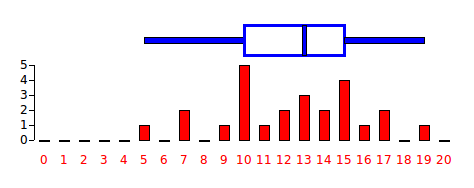
\includegraphics[scale=0.7]{ecran-stat-4}
\end{center}

Un \defi{diagramme en boîte} (appelé aussi \defi{boîte à moustaches}) est un graphique qui représente les principales caractéristiques d'une série statistique : minimum, maximum, médiane et quartiles. Le schéma de principe est le suivant :

\myfigure{0.45}{
  \tikzinput{fig-stat-boite}
} 

\newpage



\section*{Médiane et quartiles}


 Par définition, la moitié des valeurs est inférieure ou égale à la médiane, l'autre moitié est supérieure ou égale à la \defi{médiane}.

\bigskip

  \emph{Rappels.} On note $n$ la longueur de la liste et on suppose que la liste est ordonnée (du plus petit au plus grand élément).
  \begin{itemize}
    \item \textbf{Cas $n$ impair.} La médiane est la valeur de la liste au rang $\frac{n-1}{2}$.    
    
    Exemple avec \ci{liste = [12,12,14,15,19]} :
    \begin{itemize}
      \item la longueur de la liste est $n=5$ (les indices vont de $0$ à $4$),
      \item l'indice du milieu est l'indice $2$,
      \item la médiane est la valeur \ci{liste[2]}, c'est donc $14$.
    \end{itemize}
    
    \item \textbf{Cas $n$ pair.} La médiane est la moyenne entre la valeur de la liste au rang $\frac{n}{2}-1$ et au rang $\frac{n}{2}$.
    
    Exemple avec \ci{liste = [13,14,19,20]} :
    \begin{itemize}
      \item la longueur de la liste est $n=4$ (les indices vont de $0$ à $3$),
      \item les indices du milieu sont $1$ et $2$,
      \item la médiane est la moyenne entre \ci{liste[1]} et \ci{liste[2]}, c'est donc $\frac{14+19}{2} = 16.5$.
    \end{itemize}    
    \end{itemize} 


\newpage

\section*{Quartiles}

Les quartiles\index{quartiles} répartissent les valeurs en : un quart en-dessous de $Q_1$, un quart entre $Q_1$ et $Q_2$, un quart entre $Q_2$ et $Q_3$, un quart au-dessus de $Q_3$.
    Pour le calcul, on utilise que :
    \begin{itemize}
      \item $Q_2$ est simplement la médiane de la liste entière (supposée ordonnée),
      \item $Q_1$ est la médiane de la sous-liste formée de la première moitié des valeurs,
      \item $Q_3$ est la médiane de la sous-liste formée de la seconde moitié des valeurs. 
    \end{itemize}           



\newpage
   
\section*{Effectifs}   
     
Les résultats d'une classe sont collectés sous la forme suivante d'un effectif par note : \\
    \centerline{\ci{effectif_notes = [0,0,0,0,0,1,0,2,0,1,5,1,2,3,2,4,1,2,0,1,0]}} 
    Le rang $i$ va de $0$ à $20$. Et la valeur au rang $i$ indique le nombre d'élèves ayant eu la note $i$.
    
 
    Écris une fonction \ci{notes_vers_liste(effectif_notes)} qui prend en entrée un effectif de notes et renvoie la liste des notes. Pour notre exemple la fonction doit renvoyer \ci{[5,7,7,9,10,10,10,10,10,10,...]}.


\end{document}
